\documentclass[12pt]{extarticle}
\usepackage[utf8]{inputenc}
\usepackage{graphicx}
\usepackage[T2A]{fontenc}
\usepackage{geometry}
\usepackage{array}
\usepackage{graphicx}
\usepackage{setspace}
\usepackage{siunitx}
\usepackage{caption}
\usepackage{titlesec}
\usepackage[russian]{babel}
\usepackage{indentfirst}
\usepackage{setspace}
\usepackage{float}
\usepackage{array}
\usepackage{cellspace}
\usepackage{pgfplots}
\usepackage{pgfplotstable}
\usepackage{tocloft}
\usepackage{amsmath}
\usepackage{multicol}
\setlength{\cellspacetoplimit}{20pt}
\setlength{\cellspacebottomlimit}{20pt}

\onehalfspacing

\geometry{
  a4paper,
  left=30mm,
  right=20mm,
  top=20mm,
  bottom=20mm
}

\setlength{\parindent}{1.25cm}

\graphicspath{ {images/} }
\captionsetup[figure]{
  labelsep=period,
  justification=centering
}

\renewcommand{\figurename}{Рисунок}
\renewcommand{\contentsname}{Оглавление}

\titleformat{\chapter}[block]{\huge\bfseries\centering}{}{1em}{}
\titleformat{\section}[block]{\normalsize\bfseries}{\thesection}{1em}{}
\titleformat{\subsection}[block]{\normalsize\bfseries}{\thesubsection}{1em}{}
\titlespacing*{\section}{0pt}{\parskip}{-\parskip}
\titlespacing*{\subsection}{0pt}{\parskip}{-\parskip}
\titlespacing{\chapter}{0pt}{0pt}{0pt}

\renewcommand{\cftbeforetoctitleskip}{-30pt}
\renewcommand{\cftaftertoctitleskip}{-10pt}

\begin{document}

\begin{titlepage}
  \begin{center}
    \small
    \underline{
      \begin{minipage}{0.2\textwidth}
        \centering
        \includegraphics[width=3cm]{BMSTU logo}
      \end{minipage}
      \hfill
      \begin{minipage}{0.8\textwidth}
        \begin{center}

          \textbf{Министерство науки и высшего образования Российской Федерации
            Федеральное государственное бюджетное образовательное учреждение высшего образования «Московский государственный технический университет имени Н.Э. Баумана национальный исследовательский университет»
          (МГТУ им. Н.Э. Баумана)}
        \end{center}
      \end{minipage}

    }

    \vspace{7cm}
    \Large
    \textbf{Модульное домашнее задание №2} \\
    ПО ДИСЦИПЛИНЕ "Электротехника"\\
    Вариант 15\\
    \vspace{5cm}
    \normalsize
    \begin{tabular}{p{8cm}p{6cm}}
      \textbf{Студент группы ИУ1-31Б} & Соин А. Д. \\
      & «17» декабря 2025 г. \\
      & \\
      \textbf{Преподаватель} & Васюков С. А. \\
      & «\underline{\hspace{1.5cm}}»\underline{\hspace{2.5cm}}2025 г. \\
    \end{tabular}
    \vfill{\Large{Москва, 2025}}
  \end{center}
\end{titlepage}

\tableofcontents
\newpage

\section{Исходные данные}
\begin{center}
  \begin{table}[H]
    \footnotesize
    \begin{tabular}{|l|c|c|}
      \hline
      \textbf{Номинальное напряжение двигателя, В}           & $U_{\text{1н}}$                   & 220/380 \\ \hline
      \textbf{Номинальная мощность двигателя, кВт}           & $P_{\text{н}}$                    & 22      \\ \hline
      \textbf{Номинальная скорость вращения ротора, об/мин}  & $n_{\text{н}}$                    & 716     \\ \hline
      \textbf{Кратность максимального момента}               & $lambda_{\text{н}}$               & 3.0     \\ \hline
      \textbf{КПД при номинальной нагрузке, \%}              & $eta_{\text{н}}$                  & 87      \\ \hline
      \textbf{Коэффициент мощности при номинальной нагрузке} & $\cos{\phi_1}$                    & 0.82     \\ \hline
      \textbf{ЭДС заторможенного ротора, В}                  & $E_{\text{2н}}$                   & 102    \\ \hline
      \textbf{Ток ротора при номинальной нагрузке, А}        & $I_{\text{2н}}$                   & 140      \\ \hline
    \end{tabular}
  \end{table}
\end{center}

Константы
\begin{table}[H]
  \footnotesize
  \centering
  \begin{tabular}{|c|c|c|c|c|}
    \hline
    \textbf{$t$} & \textbf{$q_1$} & \textbf{$q_2$} & \textbf{$h_1$} & \textbf{$h_3$} \\ \hline
    0.8         & 0.85        & 3           & 1.05        & 0.25         \\ \hline
  \end{tabular}
\end{table}

Определим число пар полюсов двигателя по формуле $p = \frac{60f}{n_\text{н}}$ :
\begin{equation*}
  p = \frac{60f}{n_\text{н}} = \frac{60 \cdot 50}{716} = 4.19 \approx 4
\end{equation*}

Тогда частота вращения магнитного поля в асинхронном двигателе

\begin{equation*}
  n_0 = \frac{60f}{p} = \frac{60 \cdot 50 }{4} =  750 \text{об/мин}
\end{equation*}

\section{Рассчет естественных механической ($n(M)$) и электромеханической ($n(I_2)$) характеристик.}
\subsection{Механическая характеристика}

Вычислим номинальный момент двигателя
\begin{equation*}
  M_\text{н} = 9.55\frac{P_\text{н}\eta_\text{н}}{n_\text{н}} = 9.55 \frac{22000 \cdot 0.87}{716} = 255.289 \text{Нм}
\end{equation*}

Вычислим скольжение в номинальном режиме
\begin{equation*}
  s_\text{н} = \frac{n_0 - n_\text{н}}{n_0} = \frac{750 - 716}{750} = 0.047
\end{equation*}

Зная номинальный момент двигателя и кратность максимального момента, определим максимальный момент двигателя:
\begin{equation*}
  M_{max} = \lambda_kM_\text{н} = 3 \cdot 255.289 = 765.867\text{Нм}
\end{equation*}

Определим критические значения скольжения и частоты:
\begin{equation*}
  s_\text{кр} = s_\text{н}(\lambda_k + \sqrt{\lambda_k^2 - 1}) = 0.047 (3 + \sqrt{9 -1}) = 0.277
\end{equation*}
\begin{equation*}
  n_\text{н} = n_0(1 - s_\text{кр}) = 750(1 - 0.277) = 542.423 \text{об/мин}
\end{equation*}

Чтобы определить соотношение между моментом двигателя и скольжением используем формулу Клосса
\begin{equation*}
  M = \frac{2M_{max}}{\frac{s}{s_\text{кр}} + \frac{s_\text{кр}}{s}}
\end{equation*}

Связь между скоростью вращения и скольжением
\begin{equation*}
  n = n_0 (1 - s)
\end{equation*}

\subsection{Электромеханическая характеристика}

Определим угловую скорость вращения магнитного поля в двигателе
\begin{equation*}
  \Omega_0 = \frac{2\pi}{60}n_0 = \frac{2 \cdot 3.14}{60} 750 = 78.540 \text{рад/с}
\end{equation*}

Определим активное сопротивление фазы обмотки ротора:
\begin{equation*}
  R_2 = \frac{M_\text{н}\Omega_0s_\text{н}}{3I^2_{\text{2н}}} = \frac{255.289 \cdot 78.540 \cdot 0.047 }{3 \cdot 140^2} = 0.016 \text{Ом}
\end{equation*}

Для определения связи между током в обмотке ротора, моментом и скольжение используем следующую формулу
\begin{equation*}
  I_2 = \sqrt{\frac{M\Omega_0s}{3 R_2}}
\end{equation*}

\subsection{ Определение частоты вращения асинхронного двигателя, соответствующую заданному моменту нагрузки на валу}

Заданный момент нагрузки
\begin{equation*}
  M_D = t M_\text{н} = 0.8 \cdot 255.289 = 204.231 \text{Нм}
\end{equation*}

Коэффициент нагрузки при данном моменте
\begin{equation*}
  \lambda_D = \frac{M_{max}}{M_D} = \frac{579.340}{154.491} = 3.75
\end{equation*}

Найдем скольжение и частоту вращения при данном моменте

\begin{equation*}
  s_D = \frac{s_\text{кр}}{(\lambda_D + \sqrt{\lambda_D^2 - 1})} = \frac{0.277}{3.75 + \sqrt{3.75^2 - 1}} = 0.038
\end{equation*}
\begin{equation*}
  n_D = n_0(1 - s_D) = 750(1 - 0.038) = 721.813 \text{об/мин}
\end{equation*}

Значения вычисленные для построения графиков

\begin{table}[H]
  \footnotesize
  \centering
  \begin{tabular}{|l|l|l|l|l|}
    \hline
    & \textbf{s} & \textbf{n} & \textbf{M} & \textbf{$I_2$} \\ \hline
    \textbf{Холостой ход}      & 0,0000     & 750,0000   & 0,0000     & 0,0000        \\ \hline
    \textbf{}                  & 0,0100     & 742,5000   & 55,2713    & 29,8936       \\ \hline
    \textbf{}                  & 0,0200     & 735,0000   & 110,1119   & 59,6707       \\ \hline
    \textbf{Искомая точка}     & 0,0376     & 721,8128   & 204,2313   & 111,4001      \\ \hline
    \textbf{}                  & 0,0400     & 720,0000   & 216,8445   & 118,4222      \\ \hline
    \textbf{Номинальный режим} & 0,0475     & 714,3855   & 255,2891   & 140,0000      \\ \hline
    \textbf{}                  & 0,0600     & 705,0000   & 317,1554   & 175,4045      \\ \hline
    \textbf{}                  & 0,1000     & 675,0000   & 489,5283   & 281,3312      \\ \hline
    \textbf{}                  & 0,1400     & 645,0000   & 616,9489   & 373,6952      \\ \hline
    \textbf{}                  & 0,2100     & 592,5000   & 737,5801   & 500,4298      \\ \hline
    \textbf{Критический режим} & 0,2768     & 542,4233   & 765,8673   & 585,4157      \\ \hline
    \textbf{}                  & 0,3000     & 525,0000   & 763,3864   & 608,5017      \\ \hline
    \textbf{}                  & 0,4000     & 450,0000   & 716,7112   & 680,8180      \\ \hline
    \textbf{}                  & 0,5000     & 375,0000   & 649,0128   & 724,3369      \\ \hline
    \textbf{}                  & 0,6000     & 300,0000   & 582,5957   & 751,7756      \\ \hline
    \textbf{}                  & 0,7000     & 225,0000   & 523,7469   & 769,9078      \\ \hline
    \textbf{}                  & 0,8000     & 150,0000   & 473,2748   & 782,4032      \\ \hline
    \textbf{}                  & 0,9000     & 75,0000    & 430,3433   & 791,3302      \\ \hline
    \textbf{Пусковой режим}    & 1,0000     & 0,0000     & 393,7731   & 797,9064      \\ \hline
  \end{tabular}
\end{table}

Полученный график
\begin{figure}[H]
  \centering
  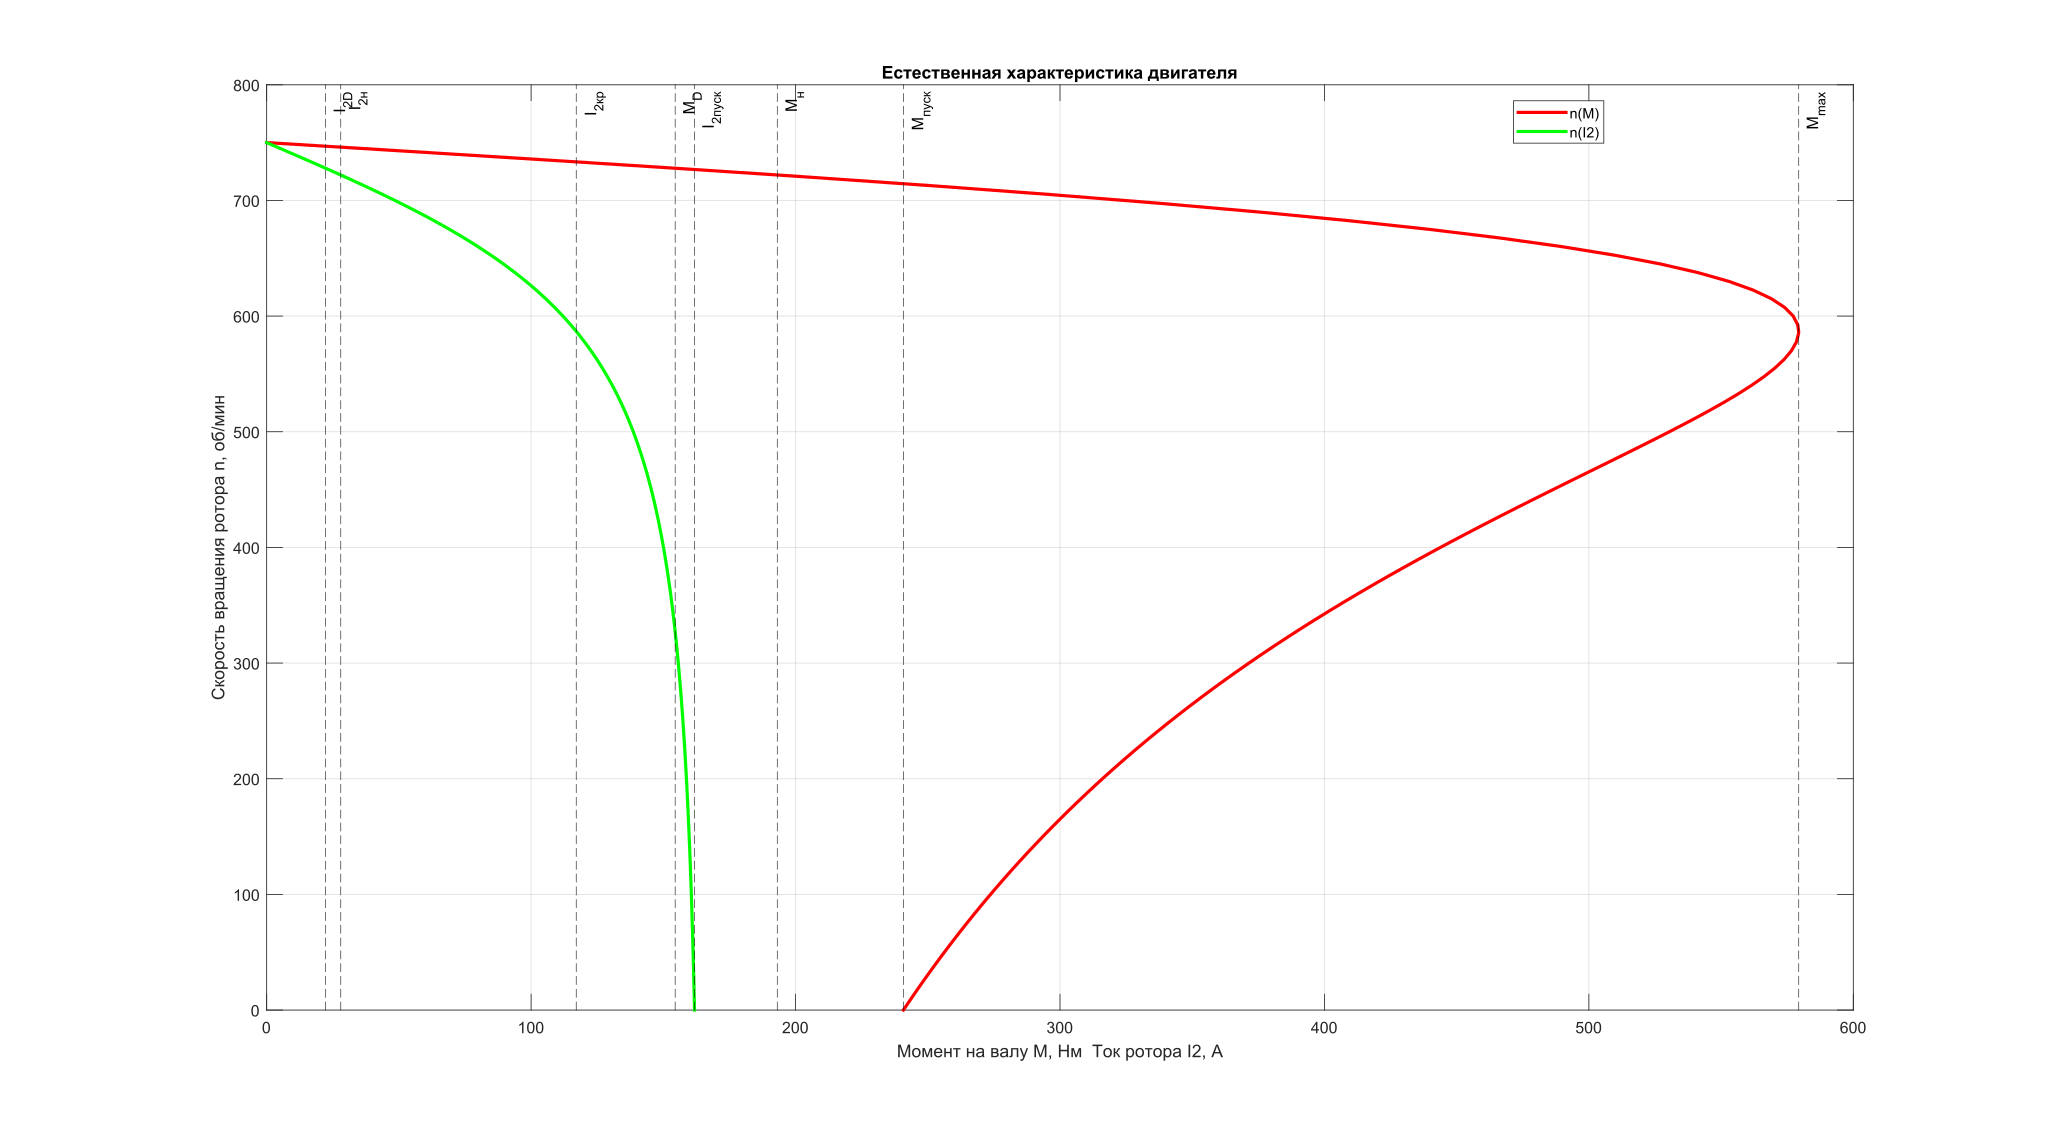
\includegraphics[width=\textwidth]{1.jpg}
  \caption{Естественные характеристики асинхронного двигателя}
\end{figure}

\section{Расчёт искусственных механических характеристик n(M) при различных способах регулирования частоты вращения трёхфазного асинхронного двигателя.}
\subsection{Рассчет механической характеристики при уменьшении напряжения источника питания}
Используя константу $q_1$  найдем механические характеристики при пониженном напряжении
\begin{equation*}
  U_1' = U_1q_1
\end{equation*}
\begin{equation*}
  M_{max}' = M_{max}q_1^2 = 765.867 \cdot 0.85 ^ 2 = 553.339
\end{equation*}
\begin{equation*}
  n_\text{кр}' = n_\text{кр} = 542.423
\end{equation*}

\begin{equation*}
  s_\text{кр}' = s_\text{кр} = 0.277
\end{equation*}
Определим коэффициент нагрузки, скольжение и скорость при данной нагрузке
\begin{equation*}
  \lambda_D' = \frac{M_{max}'}{M_D} = \frac{553.339}{204.231} = 2.709
\end{equation*}
\begin{equation*}
  s_D' =  \frac{s_\text{кр}'}{(\lambda_D' + \sqrt{\lambda_D'^2 - 1})} = \frac{0.277}{2.709 + \sqrt{2.709^2 - 1}} = 0.053
\end{equation*}
\begin{equation*}
  n_D' = n_0(1 - s_D') = 750(1 - 0.053) = 710.291 \text{об/мин}
\end{equation*}

Коэффициент регулирования
\begin{equation*}
  k_D' = \frac{n_D'}{n_D} = \frac{710.291}{721.813} = 0.984
\end{equation*}

Значения вычисленные для построения графиков

\begin{table}[H]
  \footnotesize
  \centering
  \begin{tabular}{|l|l|l|l|}
    \hline
    \textbf{}                  & \multicolumn{1}{c|}{\textbf{s'}} & \multicolumn{1}{c|}{\textbf{n'}} & \multicolumn{1}{c|}{\textbf{M'}} \\ \hline
    \textbf{Холостой ход}      & 0,0000                           & 750,0000                         & 0,0000                           \\ \hline
    \textbf{}                  & 0,0100                           & 742,5000                         & 39,9335                          \\ \hline
    \textbf{}                  & 0,0200                           & 735,0000                         & 79,5559                          \\ \hline
    \textbf{}                  & 0,0300                           & 727,5000                         & 118,5639                         \\ \hline
    \textbf{Искомая точка}     & 0,0529                           & 710,2910                         & 204.2313                         \\ \hline
    \textbf{}                  & 0,1000                           & 675,0000                         & 353,6842                         \\ \hline
    \textbf{}                  & 0,1600                           & 630,0000                         & 479,5163                         \\ \hline
    \textbf{}                  & 0,2200                           & 585,0000                         & 539,0733                         \\ \hline
    \textbf{Критический режим} & 0,2768                           & 542,4233                         & 553,3391                         \\ \hline
    \textbf{}                  & 0,3000                           & 525,0000                         & 551,5467                         \\ \hline
    \textbf{}                  & 0,4000                           & 450,0000                         & 517,8238                         \\ \hline
    \textbf{}                  & 0,5000                           & 375,0000                         & 468,9118                         \\ \hline
    \textbf{}                  & 0,6000                           & 300,0000                         & 420,9254                         \\ \hline
    \textbf{}                  & 0,7000                           & 225,0000                         & 378,4072                         \\ \hline
    \textbf{}                  & 0,8000                           & 150,0000                         & 341,9410                         \\ \hline
    \textbf{}                  & 0,9000                           & 75,0000                          & 310,9231                         \\ \hline
    \textbf{Пусковой режим}    & 1,0000                           & 0,0000                           & 284,5010                         \\ \hline
  \end{tabular}
\end{table}

Полученный график
\begin{figure}[H]
  \centering
  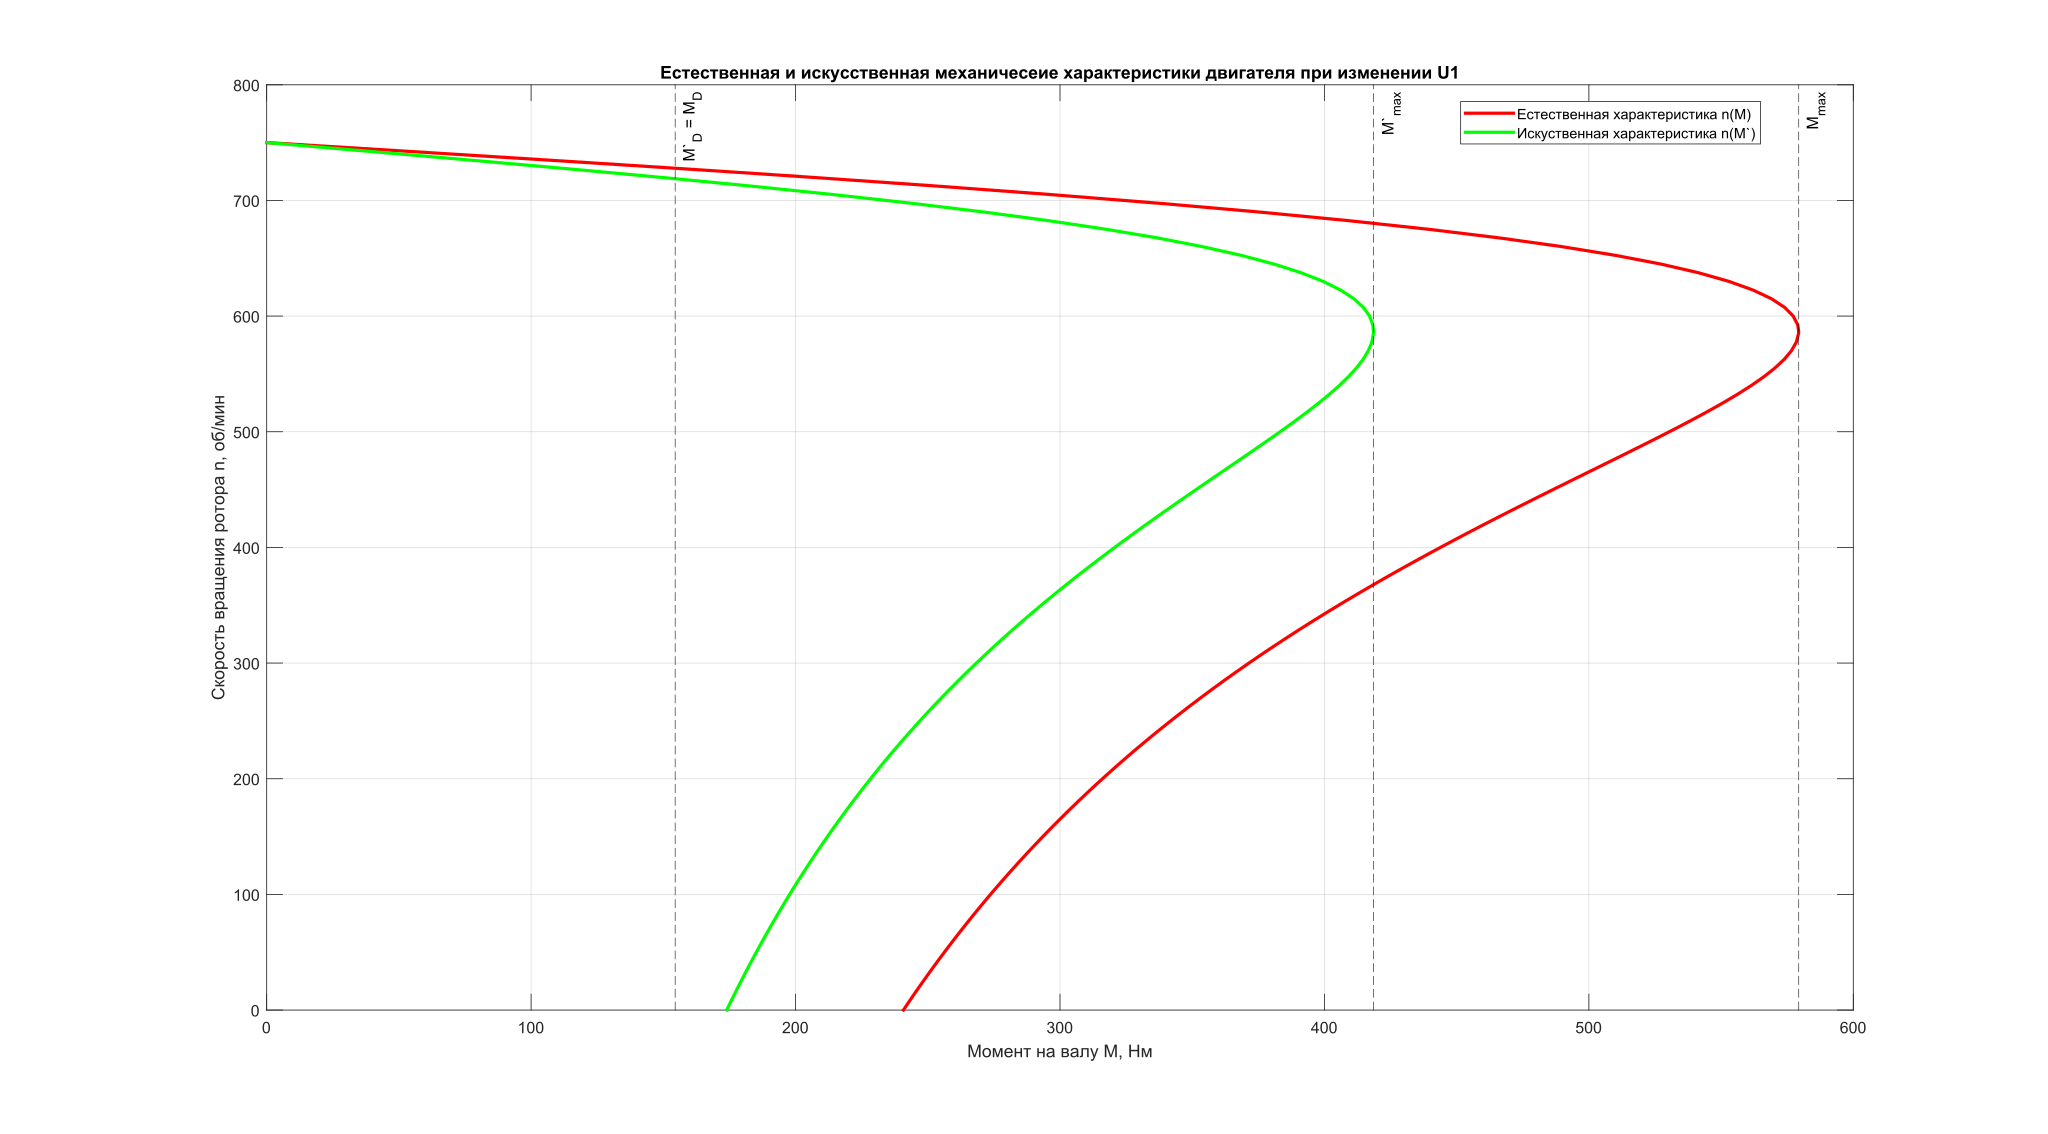
\includegraphics[width=\textwidth]{2.jpg}
  \caption{Естественная и искусственная характеристики асинхронного двигателя при изменении напряжения}
\end{figure}

Данный способ регулирования подходит для понижения  момента на валу, для  его повышения он не подходит из-за конструктивных особенностей двигателя.

\subsection{Рассчет характеристик при введении добавоного сопротивления в цепь ротора}

Добавочное сопротивление
\begin{equation*}
  R_\text{2доб} = q_2R_2 = 3 \cdot 0.016 = 0.049 \text{Ом}
\end{equation*}

Тогда
\begin{equation*}
  M_{max}' = M_{max} = 765.867
\end{equation*}

\begin{equation*}
  s_\text{кр}' = s_\text{кр} \frac{R_2'}{R_2}= 0.83
\end{equation*}

\begin{equation*}
  n_\text{кр}' = n_\text{0}(1 - s_\text{кр}')  = 127.27
\end{equation*}

Определим коэффициент нагрузки, скольжение и скорость при данной нагрузке
\begin{equation*}
  \lambda_D' = \frac{M_{max}'}{M_D} = \frac{765.867}{255.289} = 3.75
\end{equation*}
\begin{equation*}
  s_D' =  \frac{s_\text{кр}'}{(\lambda_D' + \sqrt{\lambda_D'^2 - 1})} = \frac{0.83}{3.75 + \sqrt{3.75^2 - 1}} = 0.113
\end{equation*}
\begin{equation*}
  n_D' = n_0(1 - s_D') = 750(1 - 0.113) = 665.438 \text{об/мин}
\end{equation*}

Коэффициент регулирования
\begin{equation*}
  k_D' = \frac{n_D'}{n_D} = \frac{665.438}{710.291} = 0.922
\end{equation*}

Значения вычисленные для построения графиков

\begin{table}[H]
  \footnotesize
  \centering
  \begin{tabular}{|r|l|l|l|}
    \hline
    \multicolumn{1}{|l|}{\textbf{}}                  & \multicolumn{1}{c|}{\textbf{s'}} & \multicolumn{1}{c|}{\textbf{n'}} & \multicolumn{1}{c|}{\textbf{M'}} \\ \hline
    \multicolumn{1}{|l|}{\textbf{Холостой ход}}      & 0,0000                           & 750,0000                         & 0,0000                           \\ \hline
    \textbf{}                                        & 0,0200                           & 735,0000                         & 36,8742                          \\ \hline
    \textbf{}                                        & 0,0500                           & 712,5000                         & 91,9058                          \\ \hline
    \textbf{}                                        & 0,0800                           & 690,0000                         & 146,2251                         \\ \hline
    \textbf{}                                        & 0,1100                           & 667,5000                         & 199,4258                         \\ \hline
    \multicolumn{1}{|l|}{\textbf{Искомая точка}}     & 0,1127                           & 665,4383                         & 204,2313                         \\ \hline
    \textbf{}                                        & 0,2000                           & 600,0000                         & 348,7232                         \\ \hline
    \textbf{}                                        & 0,3000                           & 525,0000                         & 489,5283                         \\ \hline
    \textbf{}                                        & 0,4000                           & 450,0000                         & 598,9149                         \\ \hline
    \textbf{}                                        & 0,5000                           & 375,0000                         & 676,9199                         \\ \hline
    \textbf{}                                        & 0,6000                           & 300,0000                         & 727,1575                         \\ \hline
    \textbf{}                                        & 0,7000                           & 225,0000                         & 754,8412                         \\ \hline
    \textbf{}                                        & 0,8000                           & 150,0000                         & 765,3382                         \\ \hline
    \multicolumn{1}{|l|}{\textbf{Критический режим}} & 0,8303                           & 127,2700                         & 765,8673                         \\ \hline
    \textbf{}                                        & 0,8700                           & 97,5000                          & 765,0330                         \\ \hline
    \textbf{}                                        & 0,9400                           & 45,0000                          & 760,0089                         \\ \hline
    \multicolumn{1}{|l|}{\textbf{Пусковой режим}}    & 1,0000                           & 0,0000                           & 752,8132                         \\ \hline
  \end{tabular}
\end{table}

Полученный график
\begin{figure}[H]
  \centering
  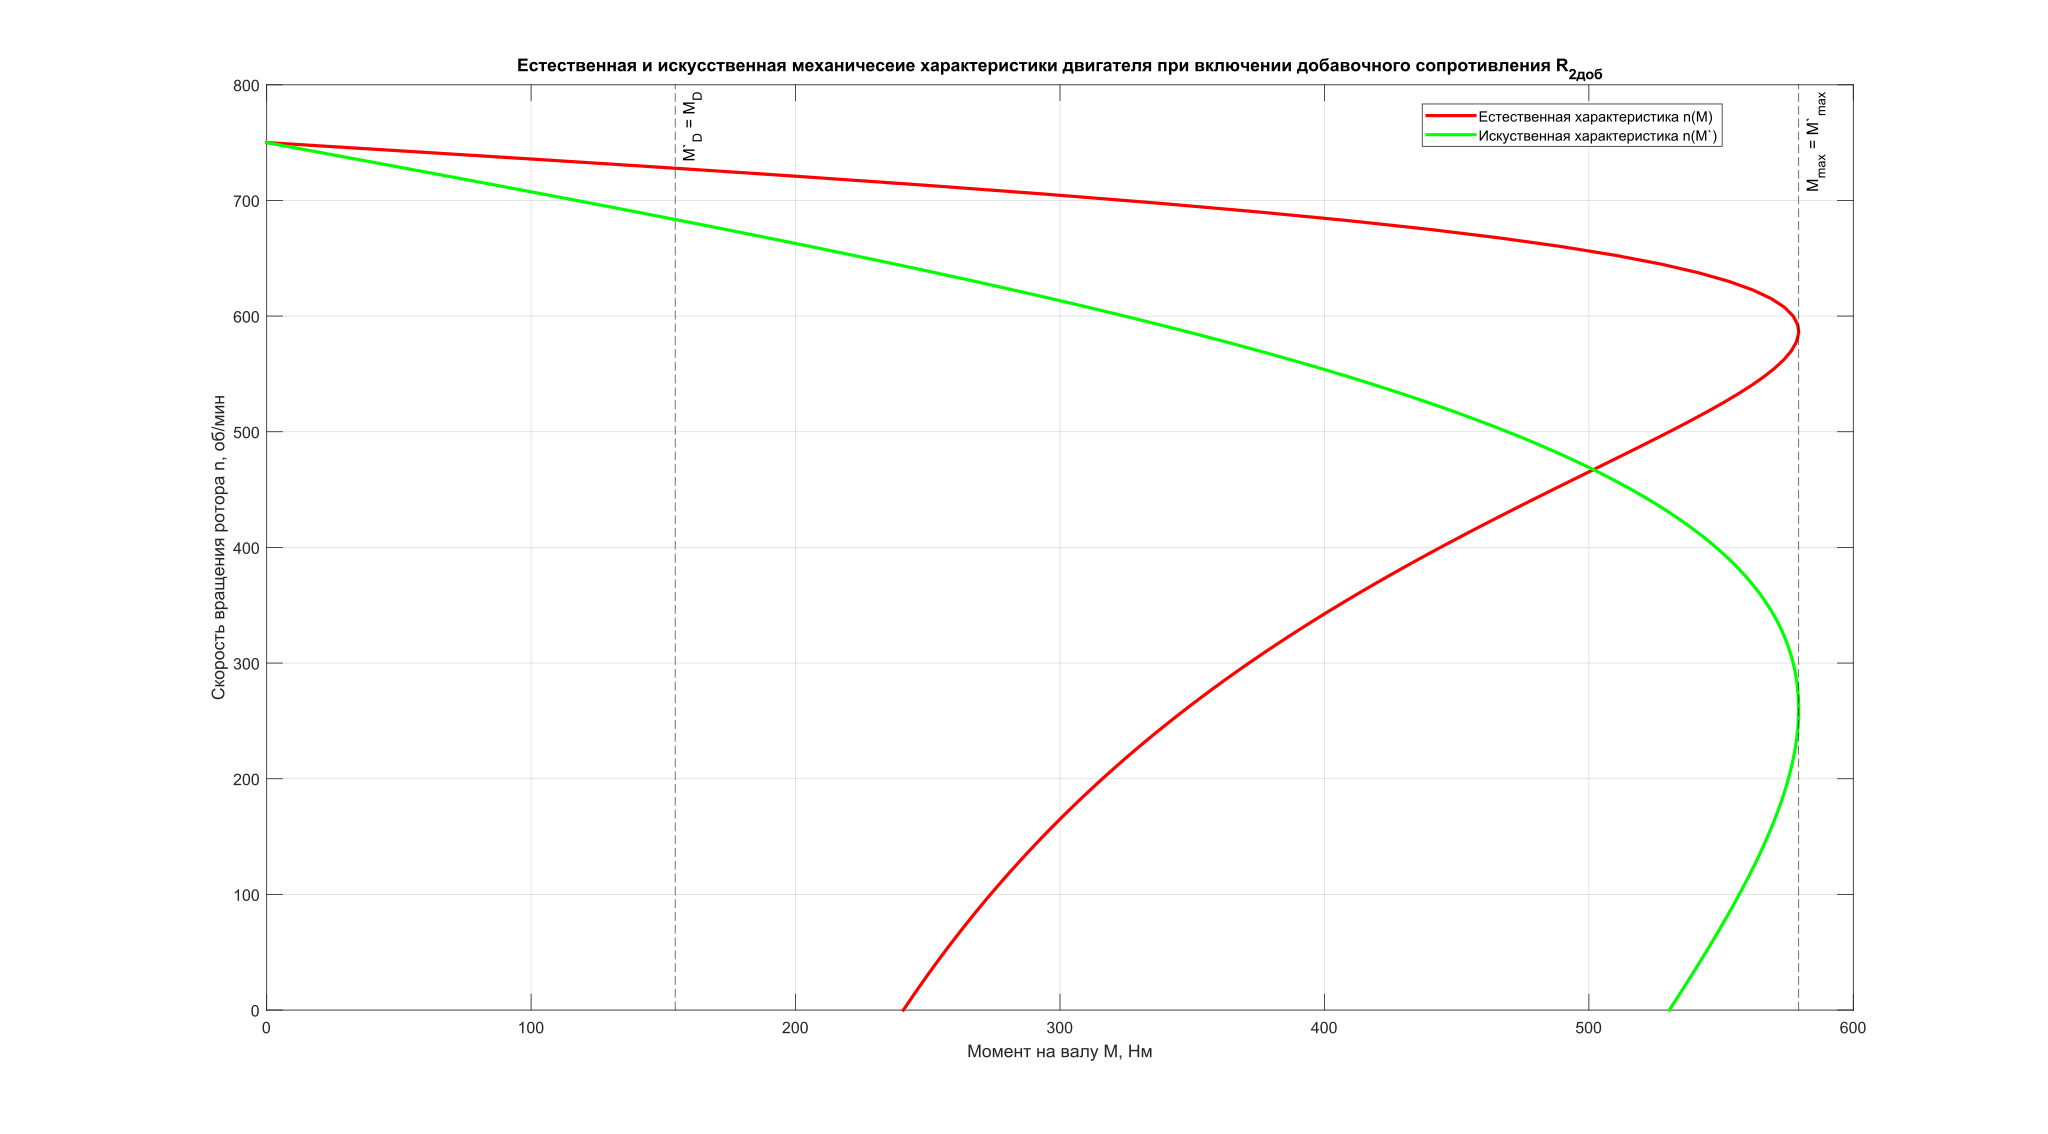
\includegraphics[width=\textwidth]{3.jpg}
  \caption{Естественная и искусственная характеристики асинхронного двигателя при включении добавочного сопротивления}
\end{figure}

Регулирование асинхронного двигателя при помощи добавления сопротивления в цепь ротора позволяет снизить скорость вращения, однако сопровождается заметным снижением КПД и ростом тепловых потерь. Этот метод целесообразен лишь для кратковременных режимов.

\subsection{Рассчет механической характеристики при изменении частоты напряжения источника питания}

Рассмотрим, как влияет изменение $f_1$ на величину момента $M_{max}$. При $U_1$=const: $M_{max}~\frac{1}{f^2}$. Обычно при регулировании частоты вращения желательно, чтобы  максимальный момент оставался неизменным. Для этого одновременно с изменением частоты напряжения необходимо  изменять и напряжение так, чтобы  выполнялось равенство $\frac{U_1}{f_1}$=const.
Определим значения изменившихся характеристик:

\begin{equation*}
  n_0' = n_0frac{f'}{f} = n_0q_1 =  750 \cdot 0.85 = 637.500 \text{об/мин}
\end{equation*}
\begin{equation*}
  \Delta n = n_0 - n_0' = 750 - 637.500 = 112.500\text{об/мин}
\end{equation*}
\begin{equation*}
  n_\text{кр}' = n_\text{кр} - \Delta n = 542.423 - 112.500 = 429.923\text{об/мин}
\end{equation*}
\begin{equation*}
  s_\text{кр}' = \frac{n_0' - n_\text{кр}'}{n_0'} = \frac{637.5 - 429.923}{637.5} = 0.326
\end{equation*}

Скорость вращения и скольжение при данном моменте

\begin{equation*}
  n_\text{D}' = n_\text{D} - \Delta n = 721.813 - 112.500 = 609.313\text{об/мин}
\end{equation*}
\begin{equation*}
  s_\text{D}' = \frac{n_0' - n_\text{D}'}{n_0'} = \frac{637.5 - 609.313}{637.5} = 0.044
\end{equation*}

Коэффициент регулирования
\begin{equation*}
  k_D' = \frac{n_D'}{n_D} = \frac{609.313}{721.813} = 0.844
\end{equation*}

Значения вычисленные для построения графиков

\begin{table}[H]
  \footnotesize
  \centering
  \begin{tabular}{|l|l|l|l|}
    \hline
    \textbf{}                  & \multicolumn{1}{c|}{\textbf{s'}} & \multicolumn{1}{c|}{\textbf{n'}} & \multicolumn{1}{c|}{\textbf{M'}} \\ \hline
    \textbf{Холостой ход}      & 0,0000                           & 637,5000                         & 0,0000                           \\ \hline
    \textbf{}                  & 0,0200                           & 624,7500                         & 93,7302                          \\ \hline
    \textbf{}                  & 0,0400                           & 612,0000                         & 185,3703                         \\ \hline
    \textbf{Искомая точка}     & 0,0442                           & 609,3128                         & 204,2313                         \\ \hline
    \textbf{}                  & 0,0500                           & 605,6250                         & 229,7912                         \\ \hline
    \textbf{}                  & 0,1100                           & 567,3750                         & 464,4545                         \\ \hline
    \textbf{}                  & 0,1700                           & 529,1250                         & 628,4164                         \\ \hline
    \textbf{}                  & 0,2300                           & 490,8750                         & 721,8139                         \\ \hline
    \textbf{}                  & 0,2900                           & 452,6250                         & 760,7590                         \\ \hline
    \textbf{Критический режим} & 0,3256                           & 429,9233                         & 765,8673                         \\ \hline
    \textbf{}                  & 0,4000                           & 382,5000                         & 749,9357                         \\ \hline
    \textbf{}                  & 0,4800                           & 331,5000                         & 711,6042                         \\ \hline
    \textbf{}                  & 0,5600                           & 280,5000                         & 665,5972                         \\ \hline
    \textbf{}                  & 0,6400                           & 229,5000                         & 619,0565                         \\ \hline
    \textbf{}                  & 0,7200                           & 178,5000                         & 575,0903                         \\ \hline
    \textbf{}                  & 0,8000                           & 127,5000                         & 534,8354                         \\ \hline
    \textbf{}                  & 0,8800                           & 76,5000                          & 498,5097                         \\ \hline
    & 0,9600                           & 25,5000                          & 465,9289                         \\ \hline
    \textbf{Пусковой режим}    & 1,0000                           & 0,0000                           & 450,9393                         \\ \hline
  \end{tabular}
\end{table}

Полученный график
\begin{figure}[H]
  \centering
  \includegraphics[width=\textwidth]{4.jpg}
  \caption{Естественная и искусственная характеристики асинхронного двигателя при изменении частоты напряжения}
\end{figure}

Метод частотного регулирования обеспечивает наибольшие возможности управления параметров двигателя, практически не изменяя форму характеристики, что делает его наиболее распространённым. Недостатком данного метода является необходимость использовать внешнее устройство – частотный преобразователь.
Если сравнивать три рассматриваемых метода регулирования скорости  асинхронного двигателя, то можно отметить, что методы понижения напряжения на источнике питания и добавления сопротивления в цепь ротора не изменяют частоту вращения магнитного поля статора, в отличии от метода частотного преобразования, обеспечивающего широкий диапазон регулирования. Кроме того, методы добавления сопротивления в цепь ротора и частотного регулирования сохраняют величину максимального момента, тогда как снижение напряжения питания приводит к его уменьшению и ухудшению перегрузочной способности двигателя.

\section{Расчёт искусственных механических характеристик при различных способах торможения трёхфазного асинхронного двигателя.}

\subsection{Генераторное торможение}

Рассмотрим работу асинхронного двигателя в режиме в тормозном режиме, на  естественной характеристике ($R_\text{доб} = 0$).

Тормозной момент
\begin{equation*}
  M_T = - t M_\text{н} = - 0.8 \cdot 255.289 = -204.231
\end{equation*}

Скорость при торможении
\begin{equation*}
  n_T = h1 n_\text{н} = 1.25 \cdot 716 = 751.800
\end{equation*}
Максимальный тормозной момент
\begin{equation*}
  M_{maxT} = - M_{max} = -765.867
\end{equation*}
Критическое скольжение
\begin{equation*}
  s_\text{крТЕ} = - s_\text{кр} =  -0.277
\end{equation*}

Коэффициент нагрузки при данном моменте

\begin{equation*}
  \lambda_D = \frac{M_{maxT}}{M_T} = \frac{ -765.867}{-204.231} = 3.75
\end{equation*}

Найдем скольжение и частоту вращения при данном моменте

\begin{equation*}
  s_\text{TE} = \frac{s_\text{крТЕ}}{(\lambda_T + \sqrt{\lambda_T^2 - 1})} = \frac{-0.277}{3.75 + \sqrt{3.75^2 - 1}} = -0.038
\end{equation*}
\begin{equation*}
  n_\text{TE} = n_0(1 - s_\text{ТЕ}) = 750(1 + 0.038) = 778.187 \text{об/мин}
\end{equation*}

Теперь рассмотрим второй этап - определение добавочного сопротивления, обеспечивающего прохождение через заданную точку  с координатам $M_T$ и $n_T$.
\begin{equation*}
  s_T = \frac{n_0 - n_T}{n_0} = \frac{750 - 751.8}{750} = -0.002
\end{equation*}
Тогда требуемое добавочное сопротивление
\begin{equation*}
  R_\text{2доб} = R2(\frac{s_T}{s_{TE}} - 1) = 0.016(\frac{-0.002}{-0.038} - 1)=  - 0.015 \text{Ом}
\end{equation*}
Критическое скольжение и скорость при прохождении через точку

\begin{equation*}
  s_\text{крT} = s_\text{крТЕ} \frac{R_2 + R_\text{2доб}}{R_2} = -0.277\frac{0.016 - 0.015}{0.16} = -0.018
\end{equation*}

\begin{equation*}
  n_\text{крT} = n_0(1 - s_\text{крT} ) = 750 (1  + 0.018) = 763.256 \text{об/мин}
\end{equation*}

Значения вычисленные для построения графиков

\begin{table}[H]
  \footnotesize
  \centering
  \begin{tabular}{|r|l|l|l|l|}
    \hline
    \multicolumn{1}{|l|}{\textbf{}}                                & \multicolumn{1}{c|}{\textbf{s}} & \multicolumn{1}{c|}{\textbf{n}} & \multicolumn{1}{c|}{\textbf{M}} & \multicolumn{1}{c|}{\textbf{M'}} \\ \hline
    \multicolumn{1}{|l|}{\textbf{Искусственная критическая точка}} & -1,5100                         & 1882,5000                       & -271,6272                       & -17,9260                         \\ \hline
    \textbf{}                                                      & -1,4000                         & 1800,0000                       & -291,4224                       & -19,3341                         \\ \hline
    \textbf{}                                                      & -1,1000                         & 1575,0000                       & -362,4512                       & -24,6046                         \\ \hline
    \textbf{}                                                      & -0,8000                         & 1350,0000                       & -473,2748                       & -33,8235                         \\ \hline
    \textbf{}                                                      & -0,5000                         & 1125,0000                       & -649,0128                       & -54,0765                         \\ \hline
    \multicolumn{1}{|l|}{\textbf{Естественная критическая точка}}  & -0,2768                         & 957,5767                        & -765,8673                       & -97,4173                         \\ \hline
    \multicolumn{1}{|l|}{\textbf{Искусственная искомая точка}}     & -0,0177                         & 763,2556                        & -97,4173                        & -765,8673                        \\ \hline
    \textbf{}                                                      & -0,0100                         & 757,5000                        & -55,2713                        & -656,4925                        \\ \hline
    \multicolumn{1}{|l|}{\textbf{Естественная искомая точка}}      & -0,0376                         & 778,1872                        & -204,2313                       & -589,8745                        \\ \hline
    \multicolumn{1}{|l|}{\textbf{Холостой ход}}                    & 0,0000                          & 750,0000                        & 0,0000                          & 0,0000                           \\ \hline
    \textbf{}                                                      & 0,1000                          & 675,0000                        & 489,5283                        & 262,5199                         \\ \hline
    \textbf{}                                                      & 0,2000                          & 600,0000                        & 727,1575                        & 134,3113                         \\ \hline
    \textbf{}                                                      & 0,3000                          & 525,0000                        & 763,3864                        & 89,9280                          \\ \hline
    \textbf{}                                                      & 0,4000                          & 450,0000                        & 716,7112                        & 67,5482                          \\ \hline
    \textbf{}                                                      & 0,5000                          & 375,0000                        & 649,0128                        & 54,0765                          \\ \hline
    \textbf{}                                                      & 0,6000                          & 300,0000                        & 582,5957                        & 45,0809                          \\ \hline
    \textbf{}                                                      & 0,7000                          & 225,0000                        & 523,7469                        & 38,6497                          \\ \hline
    & 0,8000                          & 150,0000                        & 473,2748                        & 33,8235                          \\ \hline
    \textbf{}                                                      & 0,9000                          & 75,0000                         & 430,3433                        & 30,0684                          \\ \hline
    \multicolumn{1}{|l|}{\textbf{Остановка/Пуск}}                  & 1,0000                          & 0,0000                          & 393,7731                        & 27,0636                          \\ \hline
  \end{tabular}
\end{table}

Полученный график
\begin{figure}[H]
  \centering
  \includegraphics[width=\textwidth]{5.jpg}
  \caption{Естественная и искусственная характеристики асинхронного двигателя при генераторном торможении}
\end{figure}

Метод генераторного торможения позволяет экономить энергию и обеспечивает быстрое торможение, что делает его полезным в системах, требующих точного контроля процесса остановки. Однако он требует дополнительного оборудования и может быть неэффективен для небольших двигателей или случаев, когда возврат энергии в сеть невозможен.

\subsection{Торможение противовключением}
Рассмотрим торможение противовключением с использованием реостатной характеристики

Тормозной момент
\begin{equation*}
  M_T =  t M_\text{н} =  0.8 \cdot  255.289 = 204.231
\end{equation*}

Скорость и скольжение при торможении
\begin{equation*}
  n_T =  - h3 n_\text{н} = - 0.25 \cdot 716 = -179.000
\end{equation*}

\begin{equation*}
  s_\text{T} = \frac{n_0 - n_T}{n_0} = \frac{750 + 179}{750} = 1.239
\end{equation*}

\begin{equation*}
  \lambda_T = \frac{M_{max}}{M_T} = \frac{ 765.867}{204.231} = 3.75
\end{equation*}

Критическое скольжение и скорость при торможении

\begin{equation*}
  s_\text{крT} = s_T (\lambda_T + \sqrt{\lambda_T^2 - 1}) = 1.239 ( 3.75 + \sqrt{3.75^2 - 1}) = 9.122
\end{equation*}

\begin{equation*}
  n_\text{крT} = n_0(1 - s_\text{крT} ) = 750 (1  - 9.122) = -6091.349\text{об/мин}
\end{equation*}

Добавочное сопротивление

\begin{equation*}
  R_\text{2доб} = R2(\frac{s_\text{крT}}{s_\text{кр}} - 1) = 0.016(\frac{9.122}{1.239} - 1)=  0.517 \text{Ом}
\end{equation*}

Значения вычисленные для построения графиков

\begin{table}[H]
  \footnotesize
  \centering
  \begin{tabular}{|l|l|l|l|l|}
    \hline
    \textbf{}                                & \multicolumn{1}{c|}{\textbf{s}} & \multicolumn{1}{c|}{\textbf{n}} & \multicolumn{1}{c|}{\textbf{M}} & \multicolumn{1}{c|}{\textbf{M'}} \\ \hline
    \textbf{Холостой ход}                    & 0,0000                          & 750,0000                        & 0,0000                          & 0,0000                           \\ \hline
    \textbf{}                                & 0,2500                          & 562,5000                        & 761,9220                        & 41,9485                          \\ \hline
    \textbf{}                                & 0,5000                          & 375,0000                        & 649,0128                        & 83,7086                          \\ \hline
    \textbf{}                                & 0,7500                          & 187,5000                        & 497,4994                        & 125,0945                         \\ \hline
    \textbf{Остановка/Пуск}                  & 1,0000                          & 0,0000                          & 393,7731                        & 165,9261                         \\ \hline
    \textbf{Номинальный режим}               & 1,2387                          & -179,0000                       & 325,9776                        & 204,2313                         \\ \hline
    \textbf{}                                & 2,0000                          & -750,0000                       & 207,9853                        & 320,4362                         \\ \hline
    \textbf{}                                & 3,0000                          & -1500,0000                      & 140,1196                        & 454,5905                         \\ \hline
    \textbf{}                                & 4,5000                          & -2625,0000                      & 93,8531                         & 607,7371                         \\ \hline
    \textbf{}                                & 6,0000                          & -3750,0000                      & 70,5061                         & 703,2548                         \\ \hline
    \textbf{}                                & 7,5000                          & -4875,0000                      & 56,4480                         & 751,4227                         \\ \hline
    \textbf{}                                & 8,9000                          & -5925,0000                      & 47,5873                         & 765,6353                         \\ \hline
    \textbf{Искусственная критическая точка} & 9,1218                          & -6091,3493                      & 46,4324                         & 765,8673                         \\ \hline
  \end{tabular}
\end{table}

Полученный график
\begin{figure}[H]
  \centering
  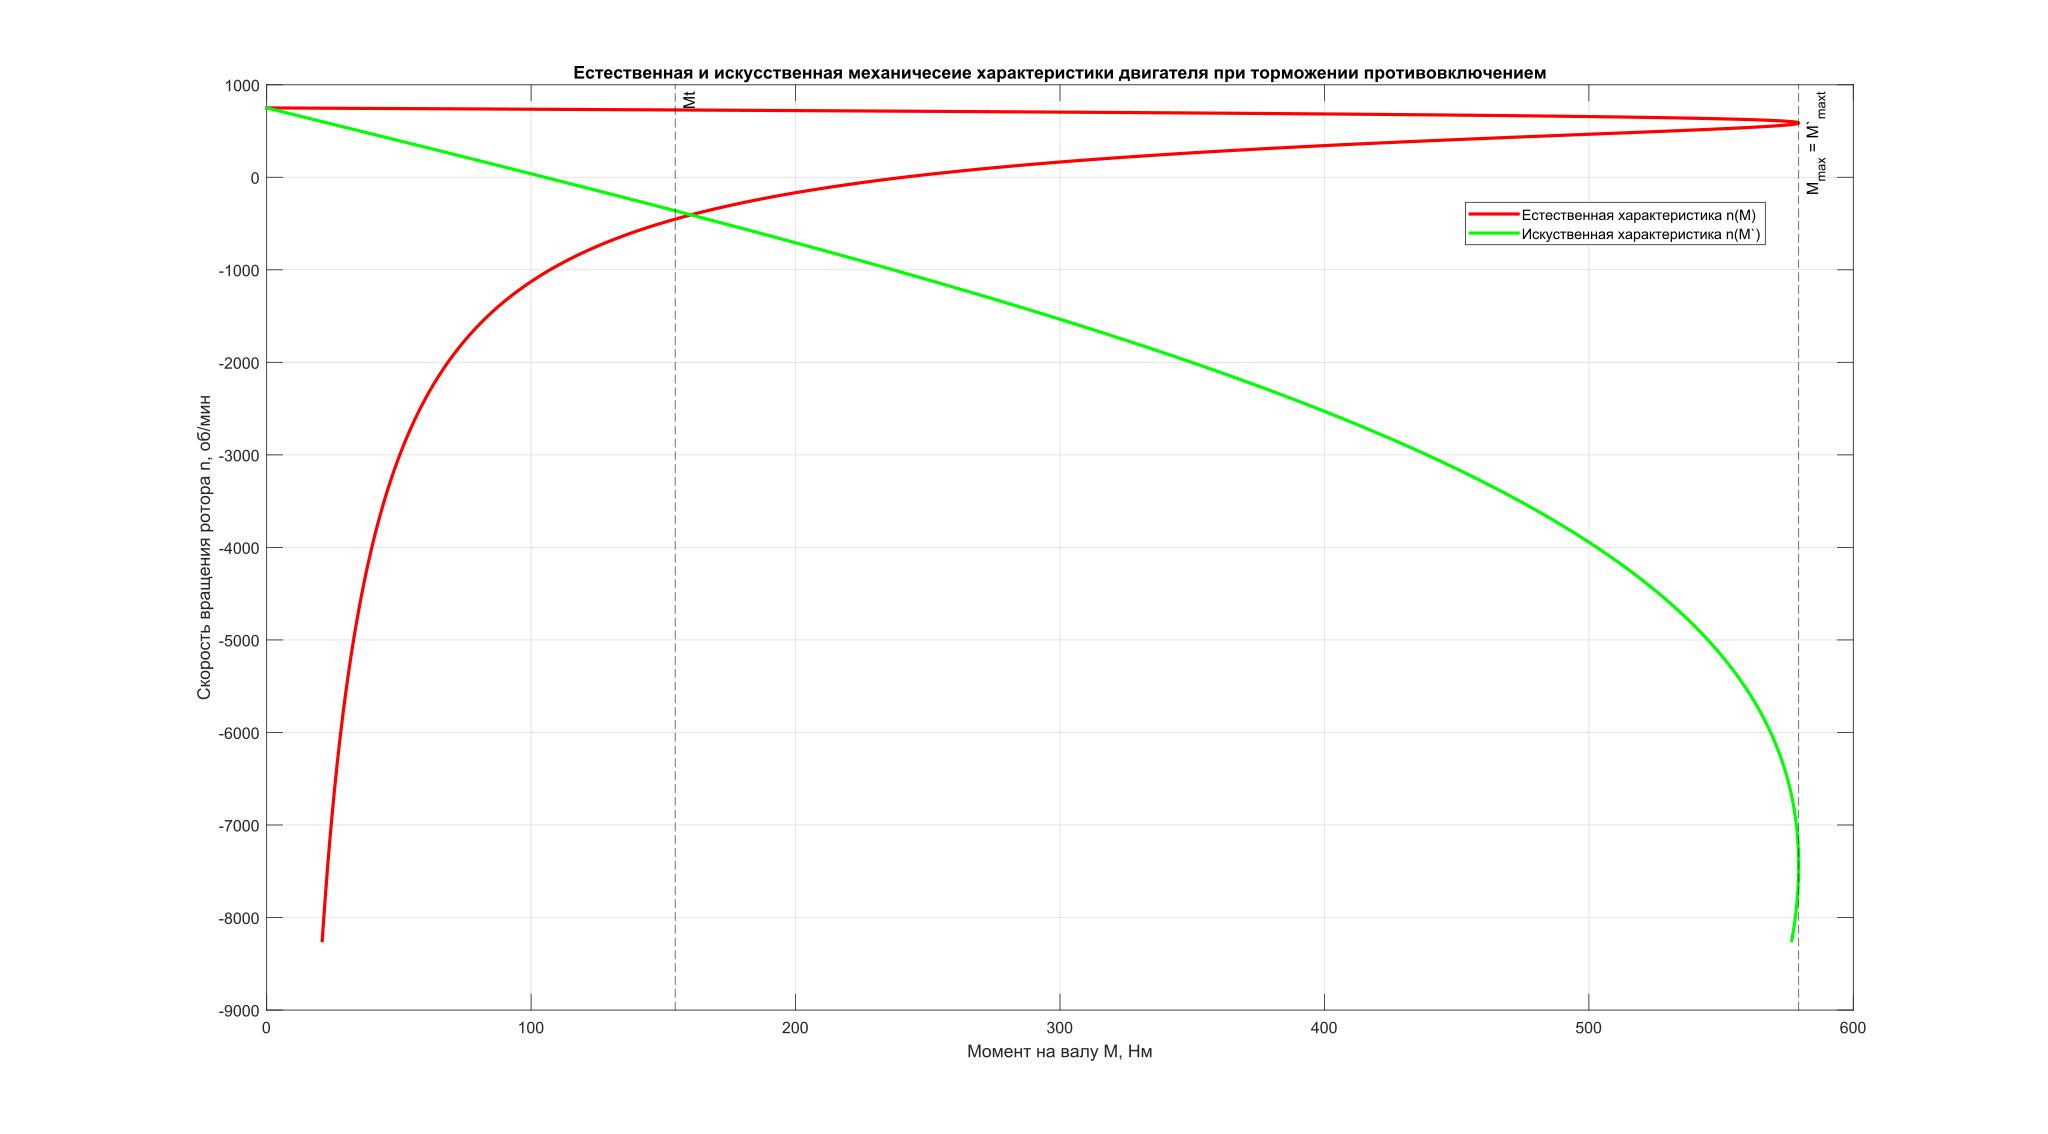
\includegraphics[width=\textwidth]{6.jpg}
  \caption{Естественная и искусственная характеристики асинхронного двигателя при торможении противовключением}
\end{figure}

Торможение противовключением отличается простотой реализации и высокой эффективностью при больших скоростях вращения, однако сопровождается значительными механическими нагрузками, повышенным тепловыделением и неэкономичным расходом энергии. Этот метод целесообразен для экстренных или аварийных режимов, где необходимо быстрое торможение, но требует учёта возможного износа и повреждения оборудования.

\end{document}